\begin{document}
	
The signal conditioner required several small changes in order to be functional. The changes are shown below in Figure \ref{fig:signalconditionerexperimentalschem}.


\begin{figure}[H]
	\centering
	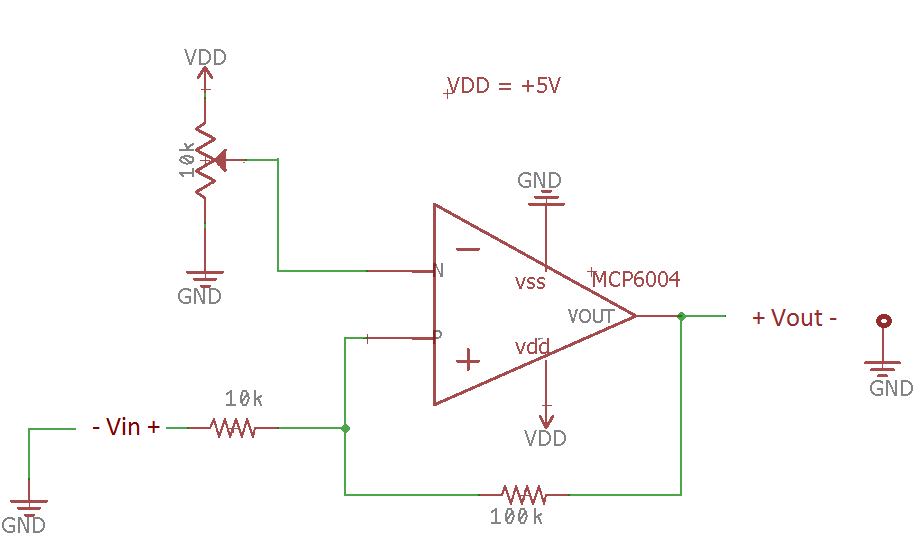
\includegraphics[width=0.65\linewidth]{ExperimentalImplementation/SignalConditionerExperimentalSchem}
	\caption{Experimental signal conditioner schematic}
	\label{fig:signalconditionerexperimentalschem}
\end{figure}

 The 100k$\Omega$ resistor voltage divider was switched to a 10k$\Omega$ potentiometer in order to facilitate easier adjustment of the output duty-cycle. The resistors in the feedback configuration were changed to 10k$\Omega$ and 100k$\Omega$. This was done in order to minimize the loading effects between the signal conditioner and the current driver. The output waveform is shown in Fig \ref{fig:conditionedvoltagelab4}.

\begin{figure}[H]
	\centering
	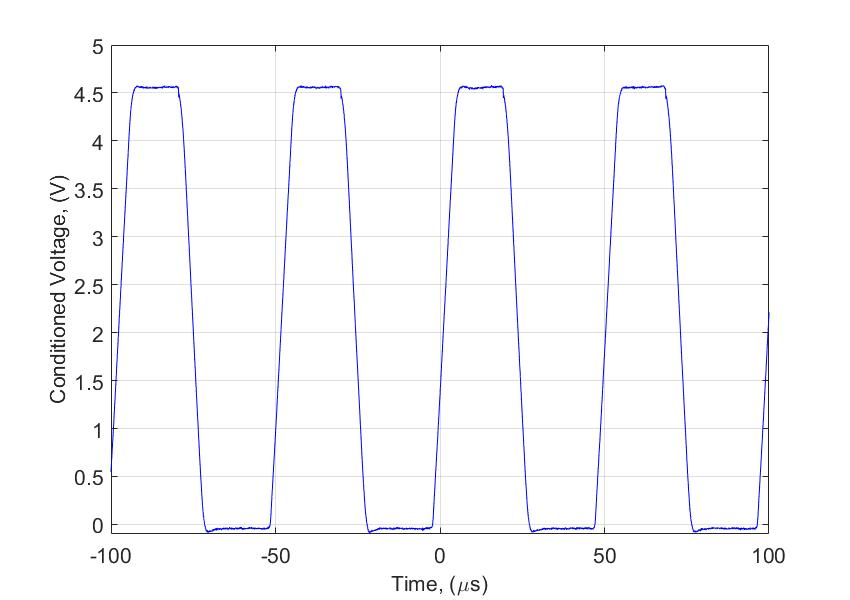
\includegraphics[width=0.6\linewidth]{ExperimentalImplementation/conditioned_voltage_lab4}
	\caption[Experimental signal conditioner]{Voltage output of signal conditioner}
	\label{fig:conditionedvoltagelab4}
\end{figure}

The output waveform operated with a 4.5V peak, 20.26kHz and 45\% duty-cycle. Table \ref{tab:currentdriver} summarizes the differences between the simulated and implemented current driver.  


\begin{table}[H]
	\centering
	\caption{Comparison of implemented driver}
	\label{tab:currentdriver}
	\begin{tabular}{|l|l|l|}
		\hline
		Component Values & Simulated  & Experimental \\ \hline
		R$_1$            & 100k$\Omega$      & 470$\Omega$        \\ \hline
		R$_2$            & 100k$\Omega$      & 1k$\Omega$      \\ \hline
		R$_{sense}$      & 12$\Omega$ & 12$\Omega$   \\ \hline
		Output current   & 200mA       & 150mA       \\ \hline
		Output current   & 200mA       & 150mA      \\ \hline
	\end{tabular}
\end{table}

Overall, the circuit required only minor changes to operate within specification.

\end{document}